\documentclass[a4paper]{memoir}
\usepackage{graphicx}
%% Language and font encodings
\usepackage{microtype}
\usepackage[paperheight=88.9mm,paperwidth=63.5mm,margin=5mm]{geometry}
\usepackage{ragged2e}
\usepackage{adjustbox}
\usepackage{emoji}
\usepackage{pgffor}
\usepackage{tikz}
\newcommand{\cardtext}{0-10}
\newcommand{\grouptext}{2-3}
\newcommand{\agetext}{12+}
\newcommand{\clocktext}{20$''$}
\newcommand{\languagecrop}{french_crop}
\newcommand{\colorcount}{4}
\newcommand{\cardtitle}{}
\def\colors{0/myyellow, 1/myorange, 2/myred, 3/mypurple}
\begin{document}
{\footnotesize
\setemojifont{NotoColorEmoji.ttf}[Path=../../../fonts/noto-emoji/]
\DeclareMicrotypeAlias{NotoColorEmoji.ttf}{TU-basic}
\newlength{\boxwidth}
\setlength{\boxwidth}{6.1mm}
\newlength{\boxheight}
\setlength{\boxheight}{9.2mm}
\newlength{\boxx}
\setlength{\boxx}{3.9mm}
\newlength{\boxy}
\setlength{\boxy}{4.3mm}
\newlength{\boxspacex}
\setlength{\boxspacex}{.4mm}
\newlength{\boxspacey}
\setlength{\boxspacey}{.4mm}
\newlength{\coldotspace}
\setlength{\coldotspace}{3.5mm}

% Define custom colors
\definecolor{myyellow}{rgb}{0.961, 0.745, 0.0}    
\definecolor{myblue}{rgb}{0.0, 0.439, 0.753}      
\definecolor{mygreen}{rgb}{0.039, 0.827, 0.376}   
\definecolor{myred}{rgb}{0.961, 0.0, 0.0}         
\definecolor{mypurple}{rgb}{0.718, 0.039, 0.718}  
\definecolor{myorange}{rgb}{1.0, 0.471, 0.039}  
\definecolor{myLighterGrey}{rgb}{0.9, 0.9, 0.9}

\begin{tikzpicture}[remember picture, overlay]
    \node[yshift=-14mm] (logo) at (current page.north)
    {
\includegraphics[width=\textwidth]{logo_alpha.png}};

    \node[yshift=1.4mm] (title) at (logo.south)
    {\cardtitle};

    \node[yshift=1.5mm, anchor=west] (qr) at (logo.west)
    {
\includegraphics[width=.267\textwidth]{qr-code.png}};

    \node[yshift=-1mm] (language) at (qr.south)
    {\adjustbox{width=.083\textwidth, height=.0498\textwidth, cfbox=black .4pt 0cm}{\includegraphics[width=.083\textwidth, height=.0498\textwidth]{../../../rule_lib/\languagecrop.png}}};

    \node[fill=myLighterGrey, xshift=-\boxx, yshift=\boxy, rounded corners, minimum width=\boxwidth, minimum height=\boxheight] (box1) at (logo.east) {};
    \node[fill=myLighterGrey, yshift=-\boxspacey-\boxheight/2, rounded corners, minimum width=\boxwidth, minimum height=\boxheight] (box2) at (box1.south) {};
    \node[fill=myLighterGrey, xshift=-\boxspacex-\boxwidth/2, rounded corners, minimum width=\boxwidth, minimum height=\boxheight] (box3) at (box1.west) {};
    \node[fill=myLighterGrey, yshift=-\boxspacey-\boxheight/2, rounded corners, minimum width=\boxwidth, minimum height=\boxheight] (box4) at (box3.south) {};

    \node[yshift=2.2mm] (cards) at (box1.center) {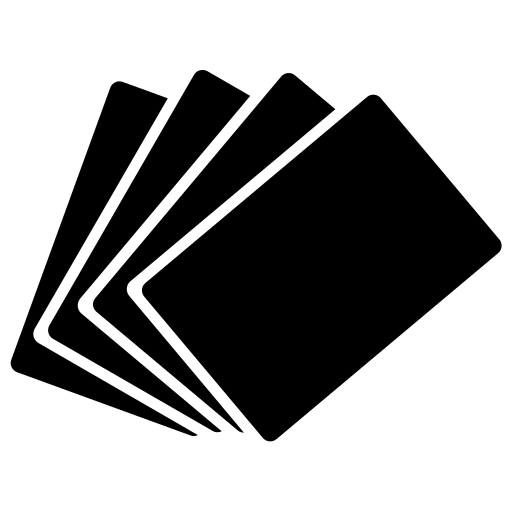
\includegraphics[width=.1\textwidth]{../../../rule_lib/cards.png}};
    \node (cards text) at (cards.south) {\cardtext};


    \foreach \i/\color in \colors {
        \ifnum \i<\colorcount
        \node[circle, fill=\color,  minimum size=3pt, scale=0.25,  xshift= (\i-.5*\colorcount+.5)*\coldotspace] (11) at (cards text.south){}; 
        \fi
    }

    \node[yshift=1.3mm] (group) at (box2.center) {
\includegraphics[width=.1\textwidth]{../../../rule_lib/group.png}};
    \node (group text) at (group.south) {\grouptext};

    \node[yshift=1.5mm] (age) at (box3.center) {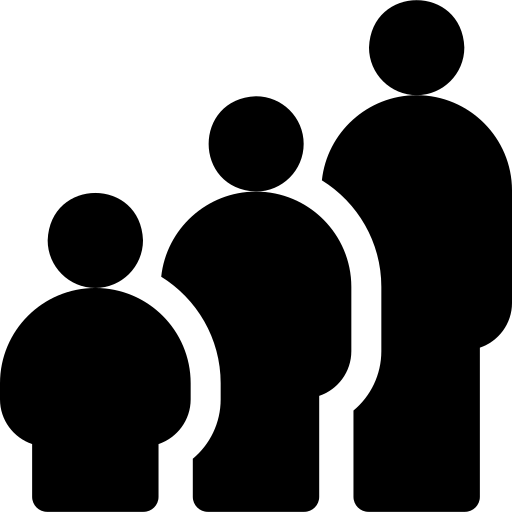
\includegraphics[width=.1\textwidth]{../../../rule_lib/age.png}};
    \node[yshift=-.5mm] (age text) at (age.south) {\agetext};

    \node[yshift=1.5mm] (clock) at (box4.center) {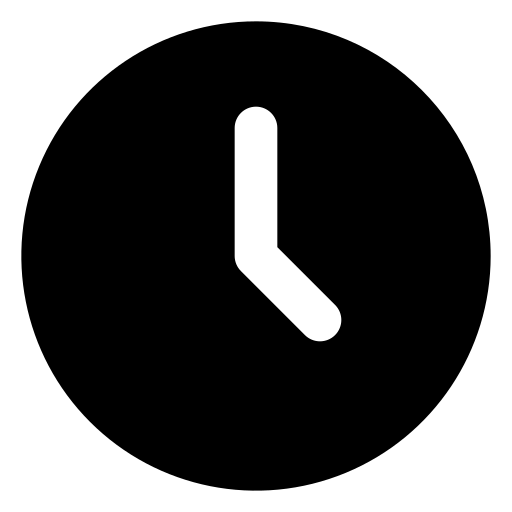
\includegraphics[width=.1\textwidth]{../../../rule_lib/clock.png}};
    \node[yshift=-.5mm] (clock text) at (clock.south) {\clocktext};
\end{tikzpicture}
\pagestyle{empty}
\justifying
$$ $$
\\
\\
\\
\\

\noindent
\textbf{\emoji{arrows-counterclockwise} Mise en place.} Mélange les cartes et distribue-les pour que chaque joueur ait une \textbf{grille de 3$\times$3 cartes face cachée}. 
Le reste des cartes forme la pioche. Retourne 2 cartes de la pioche face visible pour créer 2 défausses.
%Voilà, 3 tas de cartes bien en place au centre de la table !
\\
\\
\textbf{\emoji{game-die} Tour de jeu.} On joue à tour de rôle. À ton tour, tu dois :
\begin{itemize}
    \item \textbf{Prendre une carte} sur l'une des défausses ou en piocher une.
    \item Ensuite, utilise-la pour \textbf{remplacer} une carte de ta grille (et défausse l’ancienne) ou bien défausse-la et \textbf{retourne} une carte de ta grille.
    Avant de défausser, regarde ta carte et \textbf{choisis} bien ta défausse !
\end{itemize}
\textbf{\emoji{cross-mark} Suppression.} Dès que 3 cartes de même valeur se touchent (pas en diagonale), \textbf{elles sont défaussées (dans la défausse et dans l'ordre que tu veux)}.
\\
\\
\textbf{\emoji{stop-sign} Fin de partie.} Tes cartes sont toutes retournées ? Le jeu s'arrête pour toi. 
Les autres jouent encore une fois chacun, puis les cartes encore face cachée sont révélées.
\\
\\
\textbf{\emoji{dart} Objectif.} Avoir le \textbf{moins} de points ! 
Chaque zone de cartes de {même couleur adjacentes} vaut la valeur de la carte \textbf{la plus élevée} qu'elle contient.
Chaque \textbf{carte sombre} ajoute un point en plus.
\\
\\
\noindent
\emoji{pushpin} Mélange et/ou rééquilibre si un des 3 tas est vide.
}\end{document}